\setchapterpreamble[u]{\margintoc}
\chapter{Waves}
\labch{options}

Waves are some example of classical mechanics, where we have a function that propagates among time. During this chapter we will define their properties and their relation with quantum mechanics.

\section{The wave function}

We define a function that propagates in one dimension (x) among the time (t).

\begin{equation}
\label{wave_function}
    \psi(x,t) = e^{i(kx-\omega t)} 
\end{equation}

Where $\omega$ is the angular velocity of propagation and k is the wave number. We are working with complex numbers but the solution to the function can not be a complex number because it has a physical meaning.


We can define the phase as the function inside the exponential.

\begin{equation}
    \label{phase_def}
    \phi(x,t) = kx-\omega t
\end{equation}

If we set $\phi$ constant we will be "riding" the wave.

\section{Energy and momentum}

We are interested in see what happens among time and space in this function, so we are going to differentiate.

\begin{equation}
    \label{diff_wave}
    \begin{split}
        &\frac{d}{dt}\psi(x,t) = -i\omega e^{i(kx-\omega t)}\\
        &\frac{d}{dx}\psi(x,t) = ik e^{i(kx-\omega t)}\\
    \end{split}
\end{equation}

We choose to work with one dimension but everything could have been done in three dimensions just using x and k as vectors.

Now we are going to do some assumptions. 

\begin{equation}
    \label{Energy_Momentum}
    \begin{split}
        &E = \hbar \omega = i\hbar\frac{d}{dt}\\
        &P = \hbar k = -i\hbar\Vec{\nabla} 
    \end{split}
\end{equation}

We can define the energy as some constant ($\hbar$) times the frequency. If we use the same constant and multiply it to the wave number we get something with units of momentum, so we can call it momentum. 

The second term in both expression is what we call energy and momentum operator.  

We now from classical mechanics that energy and momentum are related.

\begin{equation}
    \label{Energy(momentum)}
    E = \frac{P\cdot P}{2m} + \nu
\end{equation}

In the previous chapter we got the expression of the energy, with which we can get the position at any time if the are some initial conditions given.

In the same way, if $\psi(\vec{x},0)$ is given we can compute $\psi(\vec{x},t)$ using the energy and momentum operators.

\section{P(x) function I: Definition and properties}

Experimentally describe a particle at rest. If we plot the position measure we will get different answers for the same experiment. 

\begin{figure}[h]
    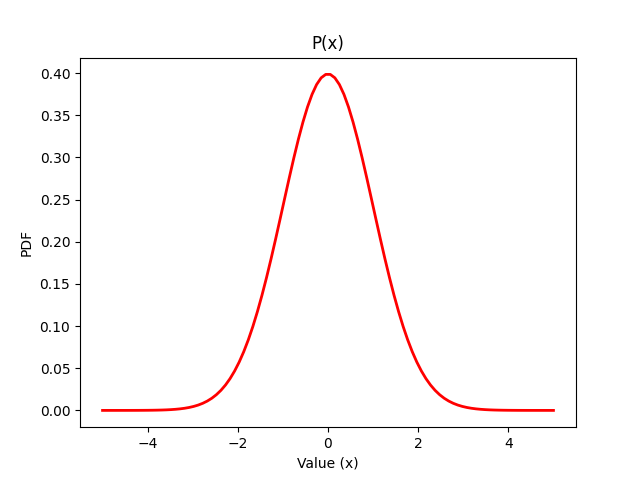
\includegraphics{images2/PDF_function.png}
    \caption{Normal distribution for mean=0 and sigma=1, to simulate a experiment measured by different people}
    \label{PDF_function}
\end{figure}
    

In wave mechanics P(x) should be interpreted as $\psi^2(x,0)$.

\marginnote[-1cm]{*Uncertainty is not probability}

We can define P(x) as a Gaussian distribution with an undetermined constant.

\begin{equation}
\label{P(x)_def}
    P(x) = A e^{-\frac{x^2}{2 \sigma^2}}
\end{equation}

We also make the next choice to define P(x):

\begin{equation}
\label{int_P(x)_def}
    \int_{-\infty}^{\infty}P(x) dx = 1
\end{equation}

We are going to ignore the constant for now to keep things simpler.

\begin{equation}
\label{int_P(x)_alpha}
    I = \int_{-\infty}^{\infty}e^{-\alpha x^2} dx 
\end{equation}

\marginnote[]{$ \Re[\alpha]> 0$, $\alpha \in \mathbb{C}$}

We need to resolve the integral of P(x), but it is not a direct integral and is difficult to resolve it directly. Luckily we can use a trick to resolve this integral.

\begin{equation}
\label{int_P(x)_r}
\begin{split}
    &I^2 = \left[\int_{-\infty}^{\infty}e^{-\alpha x^2} dx\right] \left[\int_{-\infty}^{\infty}e^{-\alpha y^2} dy\right] =\\
    & =  \int_{-\infty}^{\infty}e^{-\alpha(x^2+y^2)}dxdy = \\
    & =  \int_{0}^{2\pi}d\theta\int_{0}^{\infty}re^{-\alpha r^2}dr = \\
    & = 2\pi \frac{-1}{2\alpha} \left[ e^{-\alpha r^2} \right]_{0}^{\infty} = \frac{\pi}{\alpha}  
\end{split}
\end{equation}

\marginnote[-3cm]{dxdy = rdrd$\theta$}

If we want \ref{int_P(x)_def} to be true we need to normalize it using the result from \ref{int_P(x)_r}.

\begin{equation}
A = \sqrt{\frac{\alpha}{\pi}} \hspace{1cm} where \hspace{1cm} \alpha = \frac{1}{2\sigma^2}
\end{equation}

We get that the final value of our P(x) function is:

\begin{equation}
\label{P(x)_final_def}
    P(x) = \frac{1}{\sqrt{2\pi}\sigma} e^{-\frac{x^2}{2 \sigma^2}}
\end{equation}

We will continue with this later but first, we need to define Fourier Series.

\section{Fourier Series}

If we have a periodic function with length L so f(x) = f(x+L), then we can rewrite any function in this way:

\begin{equation}
\label{fourier}
    f(x) = \sum_{k=0}^{N} \tilde{f}_{k}\psi_{k}(x)
\end{equation}

Where $\psi_k(x)$ follow the next statements.

\begin{equation}\label{psi_k_fourier}
    \begin{split}
        &1)\hspace{2pt} \psi_k(x) = \frac{1}{\sqrt{L}}e^{i\frac{2\pi k}{L}x} \\ 
        &2) \int_0^L \psi_{k}^{\star}(x)\psi_{k'}(x) = \delta_{k,k'}
    \end{split}
\end{equation}

\marginnote[-1cm]{$\delta$ is a Dirac delta}

Using Fourier analysis we can rewrite our wave function into:

\begin{equation}
    \label{fourir_psi}
    \psi(x) = \sqrt{P(x)} = \int_{-\infty}^{\infty} \tilde{\psi}(k)e^{ikx}dk 
\end{equation}

If now we set some equations for $\psi(x)$.

\begin{equation}
    \label{rules_psi_fourier}
    \begin{split}
        &1) \hspace{2pt} Dom[\psi(x)]= \left( \frac{-L}{2},\frac{L}{2} \right) \\
        &2) \hspace{2pt} \psi(\frac{L}{2})=\psi(\frac{-L}{2})\\
        &3) \hspace{2pt} \psi(x) = e^{ikx}=e^{i\frac{2\pi n}{L}x}
    \end{split}
\end{equation}

We defined a orthogonal function $g_n$.

\begin{equation}
    \label{gn_def}
    \begin{split}
        & g_n(x) = \frac{1}{\sqrt{L}}e^{i\frac{2\pi}{L}nx}\\
        & \int_{\frac{-L}{2}}^{\frac{L}{2}}g_{n}^{\star}(x)g_{l}(x) dx = \frac{1}{L}\int_{\frac{-L}{2}}^{\frac{L}{2}} e^{i\frac{2\pi x}{L}(l-n)}dx = \delta_{l,n} 
    \end{split}
\end{equation}

\marginnote[-1cm]{$\delta_{l,n}$ is called Kronecker delta, this function is 1 when l = n and 0 for any other values}

We can use this function to rewrite $\psi(x)$

\begin{equation}
    \label{psi_gn_def} 
\begin{split}
    &\psi(x) = \frac{1}{\sqrt{L}}\sum_{n=-\infty}^{\infty}\Tilde{\psi}_n g_n(x)\\
    &\psi(x) = \frac{1}{2\pi}\sum_{n=-\infty}^{\infty} \frac{2\pi}{L}e^{i\frac{2\pi n}{L}x}\Tilde{\psi}_n
    \end{split}
\end{equation}

The last expression in \ref{psi_gn_def} is a Riemann sum so we can turn that expression into an integral.

\begin{equation}
    \label{psi_gn_final} 
\psi(x) = \frac{1}{2\pi} \int_{-\infty}^{\infty} \Tilde{\psi}(k)e^{ikx}dk
\end{equation}

We can find also an expression for $\Tilde{\psi}_n$.

\begin{equation}
    \label{til_psi_def_int} 
\begin{split}
    & \int_{\frac{-L}{2}}^{\frac{L}{2}} \psi(x) g_l^{\star}(x) dx =
    \\
    & = \frac{1}{\sqrt{L}} \sum_{-\infty}^{\infty} \Tilde{\psi}_n\int_{\frac{-L}{2}}^{\frac{L}{2}} g_n(x) g_l^{\star}(x) dx =
    \\
    & = \frac{1}{\sqrt{L}} \sum_{-\infty}^{\infty} \Tilde{\psi}_n \delta_{n,l} = \frac{1}{\sqrt{L}} \Tilde{\psi}_l
    \\
    & \Tilde{\psi}_l = \sqrt{L} \int_{\frac{-L}{2}}^{\frac{L}{2}} \psi(x) g_l^{\star}(x) dx
    \\
    & \Tilde{\psi}_l = \int_{\frac{-L}{2}}^{\frac{L}{2}} \psi(x) e^{-i\frac{2\pi l}{L}x} dx
    \end{split}
\end{equation}

If we extend to the limit where L approximate infinity we can get a general solution for $\tilde{\psi}(x)$.

\begin{equation}
    \label{2.20}
    \Tilde{\psi}(k) = \int_{-\infty}^{\infty} \psi(x) e^{-ikx} dx
\end{equation}

We have two different relations between $\psi(x)$ and $\tilde{\psi}(k)$, we need to make sure this two relations make sense together. To do this we are going to use \ref{2.20} and \ref{psi_gn_final}.

\begin{equation}
    \label{eq_2.21} 
\begin{split}
    & \psi(x) = \frac{1}{2\pi} \int_{-\infty}^{\infty} \left[ \int_{-\infty}^{\infty} \psi(y)e^{-iky}dy \right]e^{ikx}dk = 
    \\
    & = \int_{-\infty}^{\infty} \psi(y) \left[ \frac{1}{2\pi} \int_{-\infty}^{\infty} e^{ik(x-y)}dk\right]dy 
    \\
    & \psi(x) = \int_{-\infty}^{\infty} \psi(y) \delta(x-y) dy
    \end{split}
\end{equation}

The last equation we get from \ref{eq_2.21} is the definition of the Dirac delta function itself so we prove that both expressions we have are right.

\section{P(x) function II: $\psi(x)$ and $\tilde{\psi}(k)$}

We recover the equation \ref{P(x)_final_def} and know we get $\psi(x)$ remembering that $\psi^2(x) = P(x)$.

\begin{equation}
    \label{2.22}
    \psi(x) = \sqrt{P(x)} = \frac{1}{(2\pi\sigma^2)^{\frac{1}{4}} } e^{-\frac{x^2}{4\sigma^2}}
\end{equation}

We can also define $\Tilde{\psi}(k)$ with \ref{2.20}. 

\begin{equation}
    \label{2.23}
    \Tilde{\psi}(k) = \frac{1}{(2\pi\sigma^2)^{\frac{1}{4}} } \int_{-\infty}^{\infty} e^{\frac{-x^2}{4\sigma^2}-ikx}dx
\end{equation}

This integral is not easy to resolve, but we can get something similar to \ref{int_P(x)_alpha} and we already know the solution for that integral.

\begin{equation}
    \label{eq_2.24} 
    \begin{split}
    & \frac{x^2}{4\sigma^2}+ikx = \frac{1}{4\sigma^2}[x^2+4i\sigma^2 k x] = 
    \\
    & = \frac{1}{4\sigma^2}[(x+2i\sigma^2k)^2+4\sigma^4k^2]
    \\
    & e^{\frac{-x^2}{4\sigma^2}-ikx} = e^{-\sigma^2k^2}e^{-\frac{1}{4\sigma^2}(x+2i\sigma^2k)^2}
    \end{split}
\end{equation}

This expression can be used in \ref{2.23} to resolve the integral doing a variable change ($\tau = x+2i\sigma^2k$).

\begin{equation}
    \label{2.23}
    \Tilde{\psi}(k) = \frac{1}{(2\pi\sigma^2)^{\frac{1}{4}} } e^{-\sigma^2k^2} \int_{-\infty}^{\infty} e^{-\frac{\tau^2}{4\sigma^2}} d\tau
\end{equation}

\marginnote[]{We are not going to explain why $\infty+2i\sigma^2k = \infty$ and $-\infty+2i\sigma^2k = -\infty$, so the limits do not change. This can be prove with some complex analysis.}

Now we can resolve this integral because we already know the solution from \ref{int_P(x)_alpha}

\begin{equation}
    \label{2.23}
    \Tilde{\psi}(k) = \frac{1}{(2\pi\sigma^2)^{\frac{1}{4}} } e^{-\sigma^2k^2} \sqrt{4\sigma^2\pi} = 2^{\frac{3}{4}}\pi^{\frac{1}{4}}\sigma^{\frac{1}{2}} e^{-\sigma^2k^2}
\end{equation}

\section{Free particle}

If we set up the problem as a particle.

For t = 0:
    \begin{itemize}
        \item x = 0
        \item v = 0
    \end{itemize}

Then x(t) = 0. Also if E or p are given instead of v we can resolve the problem for x(t) 

If we interpret the free particle as a wave, using the knowledge from section 2.2 we will find a equation that describe the motion of the wave. First, we want to find a relation between w and k. We can get this equation using \ref{Energy_Momentum} and \ref{Energy(momentum)}. Because we are working with a free particle $\nu = 0$


\begin{equation}
    \label{2.27}
    \omega = \frac{\hbar k^2}{2m}
\end{equation}

The motion function can be found also using \ref{Energy_Momentum} and \ref{Energy(momentum)} 

\begin{equation}
    \label{2.28}
    \left(i\hbar\frac{d}{dt} \right)\psi = \frac{1}{2m}\left(-i\hbar\frac{d}{dx} \right)^2 \psi 
\end{equation}

We define P(x,0) as a gaussian function as we did in previous chapters.

\begin{equation}
    \label{2.29}
    P(x,0) = \frac{1}{\sqrt{2\pi\sigma^2}}e^{-\frac{x^2}{2\sigma^2}} 
\end{equation}

This P(x,t) function is what we called intensity of the wave, the question now is: if the wave is free ($\psi=\psi(x,t)$), what is P(x,t) ?  

We know from the previous chapter the solutions for $\psi(x,0)$ and $\Tilde{\psi}(x,0)$ when P(x,0) is a gaussian. 

\begin{equation}
    \label{2.30}
    \psi(x,0) = \frac{1}{\sqrt[4]{2\pi\sigma^2}} e^{\frac{x^2}{4\sigma^2}}
\end{equation} 

\begin{equation}
    \label{2.31}
    \tilde{\psi}(k) = 2^\frac{3}{4} \pi^\frac{1}{4} \sigma^\frac{1}{2} e^{-\sigma^2 k^2} 
\end{equation} 

If  $\psi(x,0)$ is interpreted as amplitude at x, $\tilde{\psi}(k)$ can be interpreted as amplitude at k. Also, we can define a intensity of k where $P(k) = \tilde{\psi}^2(k)$

\begin{figure}[h]
    \centering
    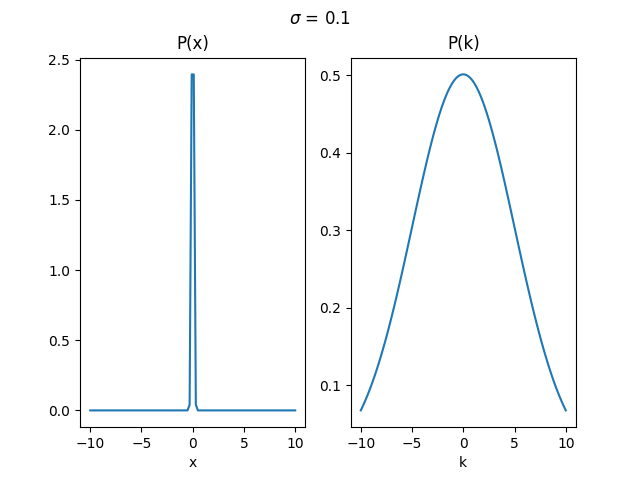
\includegraphics{images2/P_x&P_k_sigma=0.1.png}
    \caption{P(x) and P(k) for $\sigma$ = 0.1.}
    \labfig{sigma01}
\end{figure}

\begin{figure}[H]
    \centering
    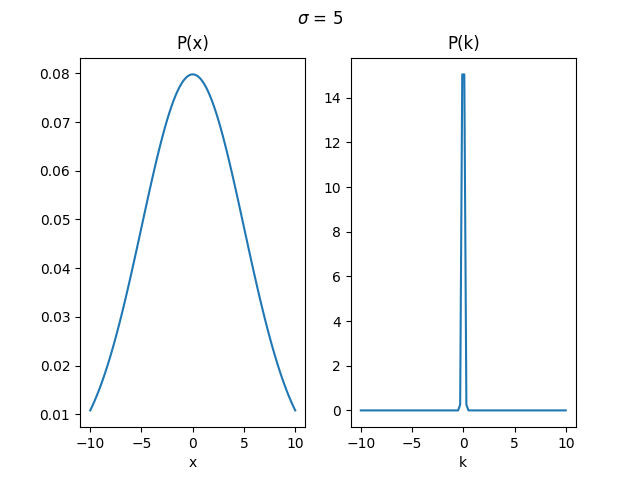
\includegraphics{images2/P_x&P_k_sigma=5.png}
    \caption{P(x) and P(k) for $\sigma$ = 5.}
    \labfig{sigma5}
\end{figure}

In this page we can see two different figures. In \reffig{sigma01} we have a very accurate result for the x value and a more deviated value for k while in \reffig{sigma5} is completely the opposite. This is a preamble to the uncertainty principle, however we still haven´t talk about quantum physics, this is just wave mechanics.


We need to get the expression among the time.

\begin{equation}
    \label{2.32}
    \psi(x,t) = \frac{1}{2\pi}\int_{-\infty}^{\infty} 2^\frac{3}{4} \pi^\frac{1}{4} \sigma^\frac{1}{2} e^{-\sigma^2 k^2} e^{ikx} e^{-i\frac{\hbar k^2}{2m}t} dk
\end{equation} 

This integral is not easy to resolve so we need to work the exponent.

\begin{equation}
    \label{2.33}
    \begin{split}
        & - \sigma^2 k^2 - i \frac{\hbar k^2}{2m} t + ikx = \\
        & = - (\sigma^2 + \frac{i\hbar t}{2m})k^2 + ikx = \\
        & = - (\sigma^2 + \frac{i\hbar t}{2m}) (k^2 - \frac{ikx}{\sigma^2 + \frac{i\hbar t}{2m}}) = \\
        & = - (\sigma^2 + \frac{i\hbar t}{2m}) (k-\frac{ix}{2(\sigma^2 + \frac{i\hbar t}{2m})})^2 + \frac{x^2}{4(\sigma^2 + \frac{i\hbar t}{2m})^2}
    \end{split}
\end{equation}

We get a similar exponent to the ones we work with where $\alpha = - (\sigma^2 + \frac{i\hbar t}{2m})$ and my variable is $\tau = k - \frac{ix}{2(\sigma^2+\frac{i\hbar t}{2m})}$

Using this to resolve \ref{2.32} we can get a final expression for $\psi(x,t)$.

\begin{equation}
    \label{2.34}
    \begin{split}
        &\psi(x,t) = \frac{1}{2\pi} 2^\frac{3}{4} \pi^\frac{1}{4} \sigma^\frac{1}{2} \frac{\pi^\frac{1}{2}}{(\sigma^2 + \frac{i\hbar t}{2m})^\frac{1}{2}} e^{\frac{-x^2}{4(\sigma^2 + \frac{i\hbar t}{2m})}} = \\
        & = \left( \frac{\sigma^2}{2\pi(\sigma^2 + \frac{i\hbar t}{2m})^2}\right)^{\frac{1}{4}}e^{-\frac{x^2}{4(\sigma^2 + \frac{i\hbar t}{2m})}}
    \end{split}
\end{equation} 

We can calculate P(x,t) knowing $\psi$(x,t).

\begin{equation}
    \label{2.35}
    \begin{split}
        & P(x,t) = \frac{\sigma}{\sqrt{2\pi}(\sigma^4 + \frac{\hbar^2t^2}{4m^2})^\frac{1}{2}}e^{\frac{-x^2}{4}\left(  \frac{1}{\sigma^2 + \frac{ikt}{2m}} + \frac{1}{\sigma^2 - \frac{ikt}{2m}}   \right)} = \\
        & = \frac{1}{\sqrt{2\pi\sigma^2(1+\frac{\hbar^2t^2}{4m^2\sigma^4})}} e^{\frac{-x^2}{2\sigma^2}\left( 
     \frac{1}{1+\frac{k^2t^2}{4m^2\sigma^4}}\right)}
    \end{split}
\end{equation} 


We can get the final result of P(x,t) from this equations.

\begin{equation}
    \label{2.36}
    P(x,t) = \frac{1}{\sqrt{2\pi \sigma^2(t)}} e^{-\frac{x^2}{2\sigma^2(t)}} 
\end{equation} 

\begin{equation}
    \label{2.37}
    \sigma(t) = \sigma\sqrt{1+\frac{\hbar^2t^2}{4m^2\sigma^4}} 
\end{equation} 

We define the characteristic time ($\tau$) as a property of the experiment itself.

\begin{equation}
    \label{2.38}
    \tau = \frac{m\sigma^2}{\hbar} 
\end{equation} 

\section{Examples}

As we did in the first chapter we want to get some real values for this equations. We will find and plot the P(x,t) and $\sigma(t)$ for 3 problems: the earth, the electron and a neutrino.

\textbf{Earth problem: } We want to measure the position of the planet earth. Our data for this problem is:

\begin{itemize}
    \item $m = 5.97 \cdot 10^{24} kg$
    \item $ \sigma_0 = 10\% $
    \item $\hbar = 1.05 \cdot 10^{-34} J/s$
\end{itemize}

We want to know the characteristic time first.

\begin{equation}
    \label{2.39}
    \tau = \frac{5.97\cdot 10^{24}\cdot 0.1^2}{1.05 \cdot 10^{-34}} = 5.69 \cdot 10^{56} s 
\end{equation}

We can plot now in steps of $\tau$ the function $\sigma(t)$.

\begin{figure}[H]
    \centering
    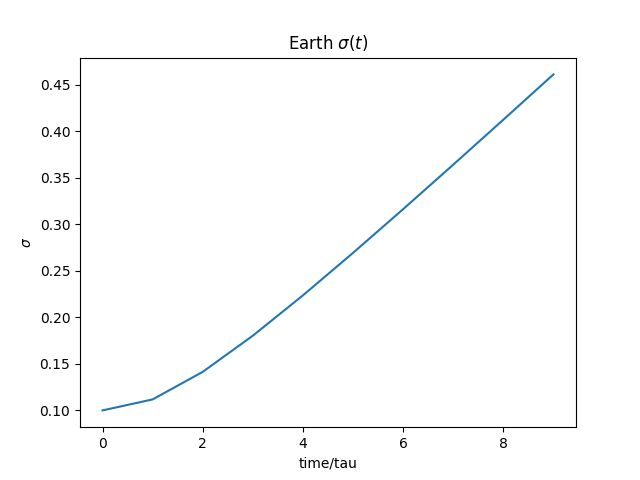
\includegraphics{images2/Earth/sigma.png}
    \caption{Function $\sigma(t)$ for the Earth experiment}
    \label{fig:sigma_earth}
\end{figure}

\begin{figure}[H]
    \centering
     \animategraphics[autoplay, loop]{4}%frame rate
    {images2/Earth/P-}%path to figures
    {0}%start index
    {19}%end index
    \caption{Gif for P(x,t) of the Earth experiment}
    \label{P_earth}
\end{figure}

\textbf{Electron problem: } We want to measure the position of an electron. Our data for this problem is:

\begin{itemize}
    \item $m = 9.11 \cdot 10^{-31} kg$
    \item $ \sigma_0 = 10\% $
    \item $\hbar = 1.05 \cdot 10^{-34} J/s$
\end{itemize}

We want to know the characteristic time first.

\begin{equation}
    \label{2.39}
    \tau = \frac{9.11\cdot 10^{-31}\cdot 0.1^2}{1.05 \cdot 10^{-34}} = 86.76 s 
\end{equation}

We can plot now in steps of $\tau$ the function $\sigma(t)$.

\begin{figure}[H]
    \centering
    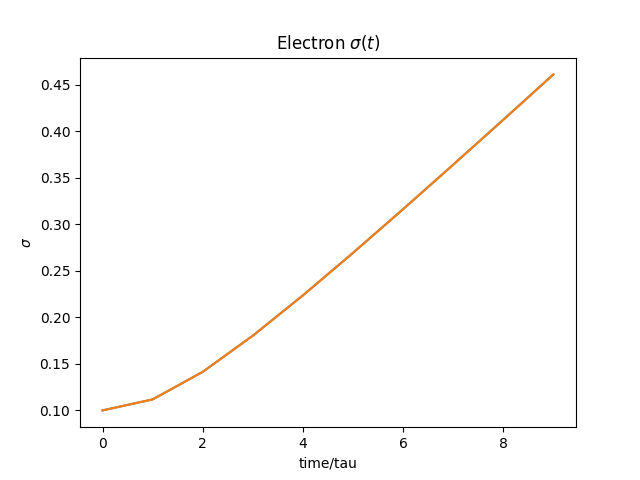
\includegraphics{images2/Electron/sigma.png}
    \caption{Function $\sigma(t)$ for the Electron experiment}
    \label{fig:sigma_electron}
\end{figure}

\begin{figure}[H]
    \centering
     \animategraphics[autoplay, loop]{4}%frame rate
    {images2/Electron/P-}%path to figures
    {0}%start index
    {19}%end index
    \caption{Gif for P(x,t) of the Electron experiment}
    \label{P_electron}
\end{figure}

At a first view the figures for the Earth and the Electron seems similar but we have to think that we are using the characteristic time as a step so the scale is completely different, while the electron functions evolve significantly in less than 100 seconds, the Earth function is changing in an order of $10^{56}$ seconds (MORE THAN THE AGE OF THE UNIVERSE!!). 


\textbf{Neutron problem: } In this experiment we are going to measure the position of a neutron before it decays. A neutron has an average life time of 879 seconds. In this case because we know the scale of time we want to work with we won't calculate the characteristic time now. The data for this experiment is:


\begin{itemize}
    \item $m = 1.67 \cdot 10^{-27} kg$
    \item $ \sigma_0 = 10\% $
    \item $\hbar = 1.05 \cdot 10^{-34} J/s$
\end{itemize}

\begin{figure}[H]
    \centering
    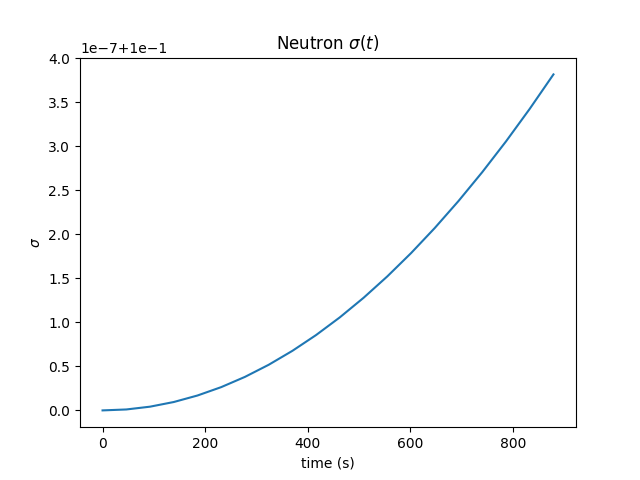
\includegraphics{images2/Neutron/sigma.png}
    \caption{Function $\sigma(t)$ for the Neutron decay}
    \label{fig:sigma_neutron}
\end{figure}

\begin{figure}[H]
    \centering
     \animategraphics[autoplay, loop]{4}%frame rate
    {images2/Neutron/P-}%path to figures
    {0}%start index
    {19}%end index
    \caption{Gif for P(x,t) of the Neutron decay}
    \label{P_neutron}
\end{figure}

In this case we can not appreciate a change in this scale of time. The neutron decays to fast to get an important change in his intensity. But how fast, is to fast? We can calculate the characteristic time to answer this question.

\begin{equation}
    \tau = \frac{1.67 \cdot 10^{-27} 0.1^2}{1.05 \cdot 10^{-34}} = 1.59 \cdot 10^5 s
\end{equation}

We can appreciate in this equation that the characteristic time is almost $10^3$ times bigger than the decay time, that is why we don't get to see a change in the density function among time.

\textbf{Extra problem: } We want to do one more experiment. We can use this functions to know how much it would change the measure of a human. The data is:

\begin{itemize}
    \item $m = 70 kg$
    \item $ \sigma_0 = 10\% $
    \item $\hbar = 1.05 \cdot 10^{-34} J/s$
\end{itemize}

We want to know the characteristic time first.

\begin{equation}
    \label{2.39}
    \tau = \frac{70\cdot 0.1^2}{1.05 \cdot 10^{-34}} = 6.67 \cdot 10^{33} s 
\end{equation}

We can plot now in steps of $\tau$ the function $\sigma(t)$.

\begin{figure}[H]
    \centering
    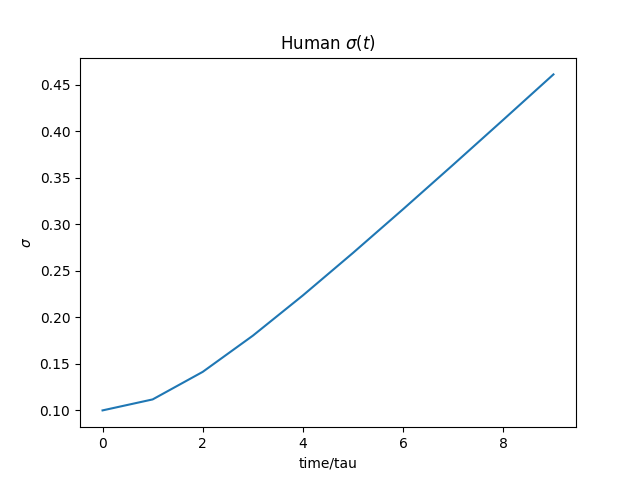
\includegraphics{images2/Human/sigma.png}
    \caption{Function $\sigma(t)$ for the Electron experiment}
    \label{fig:sigma_human}
\end{figure}

\begin{figure}[H]
    \centering
     \animategraphics[autoplay, loop]{4}%frame rate
    {images2/Human/P-}%path to figures
    {0}%start index
    {19}%end index
    \caption{Gif for P(x,t) of the Electron experiment}
    \label{P_human}
\end{figure}


Again we get something similar to the Earth and the Electron problems, but this time our step is an order of $10^{33} s$, this is still larger than the age of the universe.


A free particle is an easy example but we will start with something more difficult in the next chapter.



% In this chapter I will describe the most common options used, both the 
% ones inherited from \Class{scrbook} and the \Class{kao}-specific ones. 
% Options passed to the class modifies its default behaviour; beware 
% though that some options may lead to unexpected results\ldots

% \section{\Class{KOMA} Options}

% The \Class{kaobook} class is based on \Class{scrbook}, therefore it 
% understands all of the options you would normally pass to that class. If 
% you have a lot of patience, you can read the \KOMAScript\xspace 
% guide.\sidenote{The guide can be downloaded from 
% \url{https://ctan.org/pkg/koma-script?lang=en}.} Actually, the reading 
% of such guide is suggested as it is very instructive.

% Every \KOMAScript\xspace option you pass to the class when you load it 
% is automatically activated. In addition, in \Class{kaobook} some options 
% have modified default values. For instance, the font size is 9.5pt and 
% the paragraphs are separated by space,\sidenote[][-7mm]{To be precise, 
% they are separated by half a line worth of space: the \Option{parskip} 
% value is \enquote{half}.} not marked by indentation.

% \section{\Class{kao} Options}

% In the future I plan to add more options to set the paragraph formatting 
% (justified or ragged) and the position of the margins (inner or outer in 
% twoside mode, left or right in oneside mode).\sidenote{As of now, 
% paragraphs are justified, formatted with \Command{singlespacing} (from 
% the \Package{setspace} package) and \Command{frenchspacing}.}

% I take this opportunity to renew the call for help: everyone is 
% encouraged to add features or reimplement existing ones, and to send me 
% the results. You can find the GitHub repository at 
% \url{https://github.com/fmarotta/kaobook}.

% \begin{kaobox}[frametitle=To Do]
% Implement the \Option{justified} and \Option{margin} options. To be 
% consistent with the \KOMAScript\xspace style, they should accept a 
% simple switch as a parameter, where the simple switch should be 
% \Option{true} or \Option{false}, or one of the other standard values for 
% simple switches supported by \KOMAScript. See the \KOMAScript\xspace 
% documentation for further information.
% \end{kaobox}

% The above box is an example of a \Environment{kaobox}, which will be 
% discussed more thoroughly in \frefch{mathematics}. Throughout the book I 
% shall use these boxes to remarks what still needs to be done.

% \section{Other Things Worth Knowing}

% A bunch of packages are already loaded in the class because they are 
% needed for the implementation. These include:

% \begin{itemize}
% 	\item etoolbox
% 	\item calc
% 	\item xifthen
% 	\item xkeyval
% 	\item xparse
% 	\item xstring
% \end{itemize}

% Many more packages are loaded, but they will be discussed in due time. 
% Here, we will mention only one more set of packages, needed to change 
% the paragraph formatting (recall that in the future there will be 
% options to change this). In particular, the packages we load are:

% \begin{itemize}
% 	\item ragged2e
% 	\item setspace
% 	\item hyphenat
% 	\item microtype
% 	\item needspace
% 	\item xspace
% 	\item xcolor (with options \Option{usenames,dvipsnames})
% \end{itemize}

% Some of the above packages do not concern paragraph formatting, but we 
% nevertheless grouped them with the others. By default, the main text is 
% justified and formatted with singlespacing and frenchspacing; the margin 
% text is the same, except that the font is a bit smaller.

% As a last warning, please be aware that the \Package{cleveref} package 
% is not compatible with \Class{kaobook}. You should use the commands 
% discussed in \refsec{hyprefs} instead.

% \section{Document Structure}

% We provide optional arguments to the \Command{title} and 
% \Command{author} commands so that you can insert short, plain text 
% versions of this fields, which can be used, typically in the half-title 
% or somewhere else in the front matter, through the commands 
% \Command{@plaintitle} and \Command{@plainauthor}, respectively. The PDF 
% properties \Option{pdftitle} and \Option{pdfauthor} are automatically 
% set by hyperref to the plain values if present, otherwise to the normal 
% values.\sidenote[][*-1]{We think that this is an important point so 
% we remark it here. If you compile the document with pdflatex, the PDF 
% metadata will be altered so that they match the plain title and author 
% you have specified; if you did not specify them, the metadata will be 
% set to the normal title and author.}

% There are defined two page layouts, \Option{margin} and \Option{wide}, 
% and two page styles, \Option{plain} and \Option{fancy}. The layout 
% basically concern the width of the margins, while the style refers to 
% headers and footer; these issues will be 
% discussed in \frefch{layout}.\sidenote[][6mm]{For now, suffice it to say that pages with 
% the \Option{margin} layout have wide margins, while with the 
% \Option{wide} layout the margins are absent. In \Option{plain} pages the 
% headers and footer are suppressed, while in \Option{fancy} pages there 
% is a header.} 

% The commands \Command{frontmatter}, \Command{mainmatter}, and 
% \Command{backmatter} have been redefined in order to automatically 
% change page layout and style for these sections of the book. The front 
% matter uses the \Option{margin} layout and the \Option{plain} page 
% style. In the mainmatter the margins are wide and the headings are 
% fancy. In the appendix the style and the layout do not change; however 
% we use \Command{bookmarksetup\{startatroot\}} so that the bookmarks of 
% the chapters are on the root level (without this, they would be under 
% the preceding part). In the backmatter the margins shrink again and we 
% also reset the bookmarks root.
